\section{Megvalósítás}

Ebben a fejezetben részletesen bemutatásra kerül a rendszer megvalósítása, a projekt kezdeti létrehozásától kezdve a mappa- és fájlstruktúra leírásán át a legfontosabb funkciók implementációjáig. A cél egy átláthatóan felépített alkalmazás létrehozása, amely mind a felhasználói, mind az adminisztratív felületen stabil és könnyen karbantartható működést biztosít.

\subsection{A projekt létrehozása és környezet beállítása}

A fejlesztés Microsoft Visual Studio 2022 környezetben valósult meg, a .NET 8.0 keretrendszerre építve. A projekt típusa \textit{ASP.NET Core MVC Web Application}, amely a model-view-controller (MVC) architektúra elveit követi, lehetővé téve az üzleti logika, a megjelenítés és az adatkezelés hatékony rendszerezését.

Az adatkezeléshez az Entity Framework Core komponenst használtam, a Code First megközelítés segítségével. Az Entity Framework Core egy modern ORM( Object-Relational Mapping) technológia a .NET alkalmazások számára, amely lehetővé teszi az adatbázis-műveletek magas szintű megvalósítását. Ennek köszönhetően a modellosztályok a programkódban lettek definiálva, majd migrációk létrehozásával az adatbázis-struktúra automatikusan generálódott. Ez a módszer rugalmasságot biztosít a fejlesztés során, és egyszerűsíti az adatbázis módosítását.

Az alkalmazás egy SQL Server Express alapú relációs adatbázist használ, amely helyi környezetben gyors, megbízható és könnyen konfigurálható megoldást biztosít a fejlesztéshez. Az adatbázis kezelése teljesen az Entity Framework migrációs rendszerére épül.

\subsection{A megvalósítás mappastruktúrája és fő komponensei}

A projekt létrehozása a Visual Studio 2022 fejlesztőkörnyezet és a .NET 8 keretrendszer segítségével valósult meg. Az így generált mappastruktúra jól rendszerezett és könnyen bővíthető, támogatja az átlátható fejlesztést, és megkönnyíti az egyes komponensek logikai szétválasztását.

A \texttt{Controllers} mappa azokat az osztályokat tartalmazza, amelyek a felhasználói interakciókat kezelik és az adatokat feldolgozzák a működési logika szerint. Ezek a vezérlők külön-külön foglalkoznak az egyes entitásokkal, például a menetrendekkel, jegyekkel vagy felhasználókkal, biztosítva az adatok és a nézetek közötti kapcsolatot.

A \texttt{Models} könyvtár tartalmazza azokat az osztályokat, amelyek az adatbázisban tárolt entitásokat képezik, például a \texttt{Ticket}, \texttt{Contact} vagy \texttt{Schedule} osztályokat. Ezek az osztályok felelősek az adatok szerkezetének és az entitások közötti kapcsolatok megvalósításáért. Tulajdonképpen ezek az osztályok képezik az adatbázis tábláinak mintáját.


\subsection{Adatmodell és adatbázis felépítése}

Miután a projektet létrehoztam, elsőként az alkalmazás alapját képező osztályokat, azaz a modelleket kellett létrehozni. Ezek az osztályok az adatbázisban tárolt adattáblákat írják le, és tartalmazzák a hozzájuk tartozó tulajdonságokat, valamint az egymással kialakított relációkat. Az előzetesen elkészített adatbázis-terv alapján hoztam létre az \texttt{AdminMessage}, \texttt{AdminTask}, \texttt{Attachment}, \texttt{Bus}, \texttt{Contact}, \texttt{RouteStop}, \texttt{Schedule}, \texttt{Stop}, \texttt{Ticket}, valamint \texttt{TransportRoute} osztályokat. Fontos kritérium volt, hogy az entitások közötti relációkat pontosan és figyelmesen implementáljuk. Itt az elsődleges kulcsok (Primary Key), illetve az idegen kulcsok (Foreign Key) helyes használatára kellett különös figyelmet fordítani.

\subsubsection{Contact osztály(Identity felhasználói osztály)}

Az ASP.NET Identity rendszer egy beépített \texttt{IdentityUser} osztályt kínál, amely az alkalmazás felhasználóit reprezentálja. Ez az osztály tartalmazza az alapvető hitelesítési és azonosítási mezőket, például a \texttt{UserName}, \texttt{Email}, \texttt{PasswordHash}, \texttt{PhoneNumber} és \texttt{SecurityStamp} tulajdonságokat. Ezen mezők segítségével az Identity rendszer képes a felhasználók regisztrációját, beléptetését, valamint jelszókezelését megvalósítani.

Az osztályhoz kapcsolódóan különféle metódusokat implementálhatunk a bejelentkezéshez, jelszó reseteléshez, e-mail megerősítéshez vagy kétlépcsős hitelesítéshez. Az UserManager és SignInManager komponensek használatával közvetlenül kezelhetők a felhasználói műveletek, például új felhasználó létrehozása, jelszó validálása vagy szerepkörök hozzárendelése. Mindez könnyen implementálható, biztonságos és könnyen testreszabható felhasználókezelési rendszert biztosít a .NET alapú webalkalmazásokban.

Az alkalmazás felhasználókezelését az ASP.NET Identity keretrendszerre építettem, amely beépített mechanizmusokat biztosít a hitelesítés, az engedélyezés és a szerepkörök kezelésének megvalósításához. A rendszer egyik alapkövét a \texttt{Contact} osztály képezi, amely az \texttt{IdentityUser} osztályból származik, így örökli annak minden alapvető tulajdonságát, például a felhasználónév, e-mail, jelszóhash és biztonsági token mezőket.

Ezt az alapstruktúrát a saját igényeim szerint bővítettem ki további tulajdonságokkal, mint például a felhasználó teljes neve (\texttt{FullName}), címe (\texttt{Street}, \texttt{Zipcode}), aktív státusza (\texttt{Active}), illetve a jelszó nyers formában történő ideiglenes tárolása (\texttt{PWString}). Utóbbit a könnyebb tesztelés és használat érdekében adtam hozzá. A modell a relációs adatbázisok világához igazodva navigációs kapcsolatokat is tartalmaz más entitásokkal, például a \texttt{Ticket} vagy \texttt{Attachment} osztályokkal. (Forrás: ASP.NET Core Identity (ASP.NET Core 8.0) – Microsoft Docs)

Az ASP.NET Identity szerepköralapú jogosultságkezelést is biztosít, amely az \texttt{IdentityRole} osztályra és a felhasználókat a szerepkörökkel összekapcsoló \texttt{UserRoles} kapcsolótáblára épül. E mechanizmus révén minden felhasználó egy vagy több szerepkörhöz rendelhető, amelyek meghatározzák, milyen jogosultságokkal rendelkezik az adott rendszerben. A szerepkörök használata lehetővé teszi például, hogy az adminisztrátorok speciális funkciókhoz férjenek hozzá, míg a sima felhasználók csak az alapvető műveleteket érhetik el. A \texttt{RoleManager} szolgáltatás segítségével új szerepkörök hozhatók létre, valamint hozzárendelhetők vagy eltávolíthatók egy-egy felhasználóhoz. Ez a struktúra rugalmasan testreszabható, és könnyen beépíthető az engedélyezési logikába. (ASP.NET Core 8.0) – Microsoft Docs)



\subsubsection{AppDbContext}
Ezen felül az \texttt{AppDbContext} lehetőséget biztosít az entitások viselkedésének testreszabására az \texttt{OnModelCreating} metódusban, ahol külön definiálhatjuk a kulcsokat, kapcsolatokat, korlátozásokat, valamint egyéb konfigurációkat. Különösen hasznos az úgynevezett "vízesés törlés" (cascade delete) viselkedés figyelembe vétele, amely során egy entitás törlése vízesésszerűen magával vonhatja más kapcsolódó entitások törlését is. Az \texttt{OnModelCreating} metódus lehetőséget biztosít ennek felügyelésére, ezáltal elkerülve az adatvesztést okozó nem kívánt láncfolyamatokat, ahogy a \ref{fig:appdbcontext}. ábrán látható.  (Forrás: DbContext Configuration in EF Core – Microsoft Docs)

\begin{figure}[H]
\centering
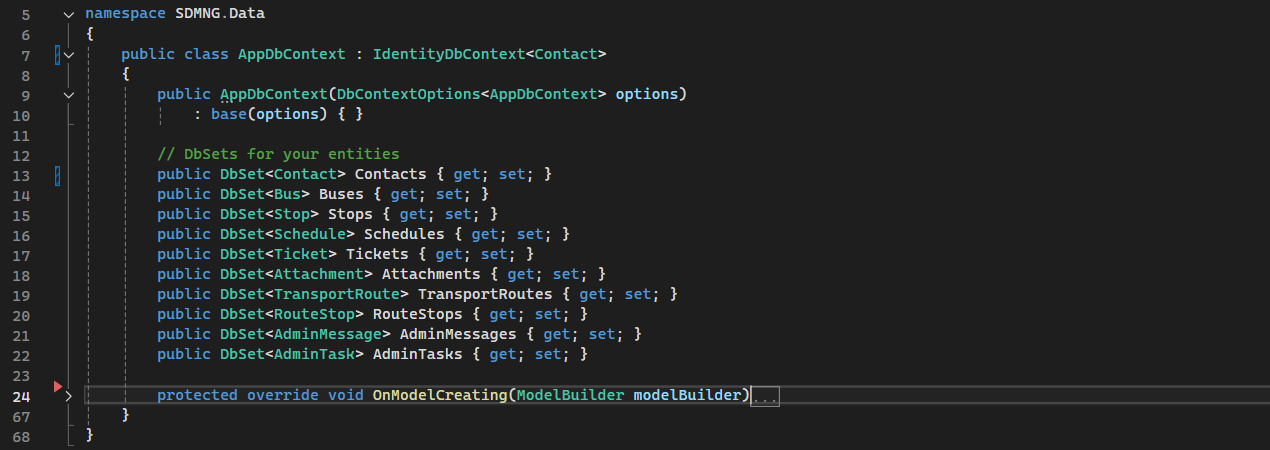
\includegraphics[width=1\textwidth]{Szakdolgozat/Mellekletek/AppDbContext.PNG}
\caption{A projektem AppDbContext osztálya látható az általam definiált modellekkel kiegészítve.}
\label{fig:appdbcontext}
\end{figure}

A \ref{fig:appdbcontext}. ábrán látható, a rendszeremben létrehozott osztályok segítségével létrehozott struktúra, amely a helyes adatbázis megvalósításában játszik kulcsszerepet. Az AppDbContext nevű osztályt az IdentityDbContext ősosztályból származtattam, majd egészítettem ki.
\vspace{\baselineskip}


Az AppDbContext osztály beállítása után szükség volt az adatbázis-fájl konfigurálására. A projekt \texttt{appsettings.json} fájlban megadtuk az adatbázis elérési útvonalát a \texttt{ConnectionStrings} szekcióban.

\begin{figure}[H]
\centering
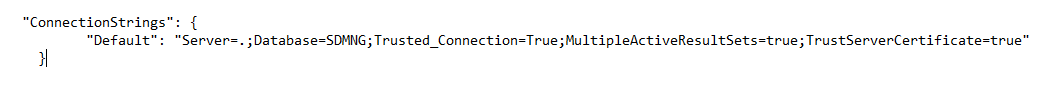
\includegraphics[width=1\textwidth]{Szakdolgozat/Mellekletek/Connectionstring.PNG}
\caption{Az adatbázis kapcsolódási kulcsa a lokális adatbázishoz.}
\label{fig:connectionstring}
\end{figure}

A \ref{fig:connectionstring}. ábrán a projektben használt \textit{connection string} látható, amely a lokális SQL Server adatbázishoz való kapcsolódást valósítja meg. Ez tartalmazza az SDMNG adatbázis elérési útvonalát, az adatbázis nevét, valamint a hitelesítési mód beállításait.
\vspace{\baselineskip}

Miután a konfigurációs fájlokat megfelelően implementáltuk, és a modellosztályaink is a tervek szerint készültek el, elérkezett az idő az első migráció létrehozására. Az adatbázis felépítését az Entity Framework migrációs rendszerével valósítottam meg. Az első migráció elkészítéséhez a terminálban a következő parancsot használtuk: dotnet ef migrations add CreateDatabase.

A parancs végrehajtása után a Migrations mappában létrejött a fentebb megadott névvel rendelkező migrációs fájl. Ezen a ponton fontos még egyszer ellenőrizni a generált adatbázis-entitásokat, és különös hangsúlyt kell fektetni a relációk helyességére. Amennyiben minden a terv szerint valósult meg, végrehajtjuk az adatbázis fizikai létrehozására vagy frissítésére szolgáló parancsot: dotnet ef database update.

Ez a parancs a korábban generált migrációs fájlok alapján felépíti vagy kiegészíti az adatbázist a megadott kapcsolati karakterlánc (connection string) segítségével.

\subsection{Vezérlők (Controllers) felépítése és működése}
Az alkalmazás működésének egyik kulcseleme a vezérlők rendszere. Ezek azok az osztályok, amelyek közvetlen kapcsolatban állnak a felhasználóval: fogadják az oldalkéréseket, előkészítik az adatokat, és eldöntik, milyen nézetet kell megjeleníteni vagy milyen műveletet kell végrehajtani. A vezérlők az MVC architektúra "C" komponensét képviselik, tehát az alkalmazás logikai magját képezik.

A projektben minden jelentősebb funkció – például jegyvásárlás, menetrendkezelés, felhasználói adatok kezelése – külön vezérlőt kapott. Ezek az osztályok a \texttt{Controllers} nevű mappában találhatóak, és  a \texttt{Controller} alaposztályból öröklődnek.

\subsubsection{A konstruktor szerepe}
A vezérlők konstruktorában történik meg az úgynevezett függőséginjektálás (dependency injection). Ez azt jelenti, hogy a vezérlő induláskor automatikusan megkapja azokat a szolgáltatásokat vagy komponenseket, amelyekre működése során szüksége lesz – például az adatbázis-kapcsolatot biztosító \texttt{AppDbContext} példányt.

\subsubsection{Aszinkron metódusok (async/await)}
A vezérlők fejlesztése során aszinkron metódusok használtam. Ennek elsődleges oka, hogy ezek a metódusok hatékonyabb működést tesznek lehetővé, különösen akkor, amikor a rendszer külső erőforráshoz – például adatbázishoz – fordul adatlekérés vagy módosítás céljából. Ilyen esetekben a programnak várnia kell a válaszra, és ha ez a várakozás egy szinkron módon írt metódusban történik, az idő alatt az egész kérés „lefagyhat”, nem képes más feladatokra reagálni.

Az aszinkron működés lényege, hogy ezek a metódusok nem akadályozzák az alkalmazás többi részének futását, miközben például háttérben adatokat kérnek le vagy dolgoznak fel. Ez különösen fontos egy webalkalmazás esetén, ahol egyszerre több felhasználói kérés is érkezhet – például jegyvásárlás, menetrend megtekintés vagy felhasználói adatok kezelése. Az \texttt{async/await} kulcsszavak használatával ezek a műveletek párhuzamosan, egymást nem akadályozva tudnak végbemenni.

Az aszinkron működés megvalósításában kulcsszerepet játszik két kifejezés: az \texttt{async} és az \texttt{await}. Az \texttt{async} kulcsszóval azt jelezzük a rendszernek, hogy az adott metódus tartalmazhat olyan műveleteket, amelyek végrehajtása hosszabb időt vesz igénybe, és ezeket érdemes nem blokkoló módon kezelni. Ezzel előkészítjük a metódust arra, hogy akár több lépésben, megszakítható módon fusson le.

Az \texttt{await} pedig azt mondja a programnak, hogy itt most egy időigényes művelet következik – például adatbázis-lekérdezés vagy fájl beolvasása –, és a vezérlés addig adódjon vissza a hívó félnek, amíg ez be nem fejeződik. A lényeg az, hogy a várakozás ideje alatt a többi feladat nem áll meg, az alkalmazás közben más kéréseket is képes kiszolgálni.

Egy-egy metódus így nemcsak hatékonyabb, de a felhasználói élményt is képes pozitívan befolyásolni, mivel csökken a válaszidő, gyorsabban jelennek meg az oldalak, és kevesebb az esély a hibákra vagy „megakadásokra”. A projekt során ezért az adatbázissal kapcsolatos lekérdezések és módosítások szinte minden esetben aszinkron módon lettek megvalósítva.

\subsubsection{Hibakeresés, csatolmánykezelés}
Az alkalmazás készítése közben nagyon fontos szerepet kapott a naplózás és a környezeti beállítások kezelése, mert ezek segítenek gyorsan megtalálni a hibákat és biztosítják, hogy a rendszer megbízhatóan működjön. A fejlesztés során az ASP.NET Core beépített \texttt{ILogger} felületét használtam, ami egy hatékony eszköz a különféle események naplózására. Ez azt jelenti, hogy az alkalmazás működésével kapcsolatos fontos információkat — például figyelmeztetéseket vagy hibákat — eltárolhatjuk, így könnyebben nyomon követhető, mi történik a háttérben, és gyorsan rá lehet jönni, ha valami nem működik jól.

Az \texttt{ILogger} segítségével például a fájlok feltöltésekor vagy e-mail küldéskor felmerülő hibák részletesen naplózhatóak, így visszakövethetővé válik, hogy mikor és milyen körülmények között jelentkezett az adott hiba. Ez különösen hasznos fejlesztési és tesztelési fázisban, amikor az alkalmazás viselkedését pontosan felügyelni kell.

A csatolmányok feltöltésekor az \texttt{IWebHostEnvironment} segítségével meghatároztam a fájlok fizikai tárolási helyét, amely általában a \texttt{wwwroot/} mappában található. Ez a megközelítés lehetővé teszi, hogy a különböző környezetekben eltérő útvonalakat használjunk, megkönnyítve ezzel a fejlesztést és a telepítést. A feltöltött fájlok elérését pedig dinamikusan, az alkalmazás futási környezetétől függően kezeljük.
\subsubsection{Regisztráció és felhaszálói szerepkör menedzselési komponensek}
A \texttt{Contact} osztályra épülő hitelesítési és regisztrációs funkciók az \texttt{AccountController} osztályon belül valósítottam meg. Ezen funkciók szétválasztását a Contact controllertől azért láttam fontosnak, mivel itt a kontakt osztály metódusai vannak definiálva a személyes fiókr nézve. A ContactControllerben viszont az admin funkciók kerültek megvalósításra az összes kontact számára. Ez jol strukturált felépítést eredményez, valamint megkönnyíti a kiegészítést, ejlesztést. 

Az \texttt{Account} vezérlő működését két fontos Identity-komponens, a UserManager<TUser> és a \texttt{SignInManager<TUser>} segíti. A \texttt{UserManager} az általános felhasználókezelési műveletekért felelős, mint például új felhasználó létrehozása, jelszó módosítása, szerepkörök kezelése, míg a \texttt{SignInManager} a be- és kijelentkezés lebonyolítását végzi.

A regisztráció során a rendszer egy új \texttt{Contact} példányt hoz létre a megadott adatok alapján, majd a \texttt{UserManager.CreateAsync()} metódussal menti azt az adatbázisba. A sikeres regisztrációt követően a felhasználó automatikusan hozzá van rendelve egy alapértelmezett szerepkörhöz (pl. \texttt{"User"}), amit a \texttt{UserManager.AddToRoleAsync()} metódus hajt végre. Ez lehetővé teszi a későbbi gördülékeny engedélykezelést, például admin jogosultságok bevezetését vagy jogosultságok szűrését nézetek szerint.

A bejelentkezés folyamata a \texttt{SignInManager.PasswordSignInAsync()} metódus segítségével valósul meg, amely ellenőrzi a megadott hitelesítési adatokat és elvégzi a bejelentkeztetést, ha azok helyesek. Hibás adatok esetén a rendszer visszajelzést ad a felhasználónak, ezáltal a folyamat megismétlése vagy ennek változtatásának lépése következik.

A \texttt{ChangePassword} és \texttt{VerifyEmail} akciók külön lehetőséget biztosítanak a felhasználóknak arra, hogy hitelesített módon módosítsák jelszavukat. Az e-mail cím ellenőrzését követően a jelszó eltávolítása és újra beállítása a \texttt{UserManager.RemovePasswordAsync()} és \texttt{AddPasswordAsync()} metódusokkal történik, ezzel biztosítva a jelszavak érvényességének újradefiniálását.

Végezetül a \texttt{Logout} akció gondoskodik a hitelesítési cookie érvénytelenítéséről és a felhasználó kijelentkeztetéséről a \texttt{SignInManager.SignOutAsync()} metódus segítségével, biztosítva ezzel a biztonságos felhasználói munkamenetek lezárását.

Ez a megoldás egyrészt jelentősen leegyszerűsíti a hitelesítési logika implementálását, másrészt rugalmasan bővíthető a jövőbeni funkciók igényei szerint – például kétfaktoros azonosítás, e-mail megerősítés vagy jogosultságszintek kialakítása. A \texttt{Contact} modell és a hozzá tartozó Identity szolgáltatások közösen biztosítják az alkalmazás integrált, skálázható és biztonságos felhasználókezelését.


\subsubsection{Biztonság és hitelesítés a vezérlők szintjén}
A vezérlők kialakításakor különös figyelmet fordítottam a biztonsági elvekre. Az ASP.NET Identity keretrendszer biztosította a hitelesítés és szerepkör-alapú jogosultságkezelés infrastruktúráját. Az alkalmazásban minden vezérlő és metódus, amely érzékeny adatot kezel vagy kizárólag regisztrált felhasználók számára elérhető, az \texttt{[Authorize]} attribútummal van ellátva. Egyes metódusoknál szerepkörhöz kötött elérés is alkalmazásra került, például az adminisztrációs felületek esetében kizárólag az Admin szerepkörrel rendelkező felhasználók végezhetnek műveleteket.

A \texttt{[Authorize]} attribútum legfontosabb megjelenési formája a bejelentkezés utáni jogosultság-kezelés: amennyiben a felhasználó nem azonosította magát, vagy nem rendelkezik a megfelelő szerepkörrel, nem férhet hozzá bizonyos oldalakhoz és műveletekhez. Ezáltal biztosítható, hogy például az adminisztrátor által elérhető listázási, szerkesztési vagy törlési funkciókat egy egyszerű, be nem jelentkezett felhasználó ne láthassa vagy használhassa.

A jelszavak kezelése az ASP.NET Identity rendszer beépített funkcióin keresztül történik, amely a felhasználói jelszavakat biztonságos módon, hashing algoritmus alkalmazásával tárolja az adatbázisban. A jelszavak visszafejtése nem lehetséges, csak a hash-értékek kerülnek mentésre. Ez alapértelmezett védelem a jogosulatlan hozzáférés ellen, még akkor is, ha valaki illetéktelenül hozzájutna az adatbázishoz.

\subsection{Fontosabb kontrollermetódusok megvalósítása}
\subsubsection{JegyController metódusok (Ticket)}
A fejlesztés során több olyan vezérlőmetódus valósúlt meg, amelyek összetettebb funkciókat látnak el, például a jegyvásárlási folyamat kezelését. Ez magában foglalja a vásárlás rögzítését, a QR-kód generálását, valamint a felhasználó számára történő visszaigazolást e-mail formájában.

A jegyvásárlási folyamat egyik fontos lépése a QR-kód generálása, a \ref{fig:attach-qr-send-email}. ábrán bemutatott részlet szemlélteti, amely egy útvonalat tárol, pontosabban egy URL-t tartalmaz, amely a webalkalmazás adott oldalára — például a jegy részleteit bemutató Ticket Detail oldalra — mutat. Ez az URL tartalmazza a jegy egyedi azonosítóját, így a QR-kód beolvasásakor a felhasználó közvetlenül a megfelelő oldalra jut. A QR-kód generálása általában egy erre alkalmas, külső könyvtár vagy csomag segítségével történik, amely az URL-t vizuális, képi formátumba alakítja át (például PNG formátumú képpé), és ezt a képet az alkalmazás vagy az e-mail csatolmányaként használja fel.

\begin{figure}[H]
\caption{QR-kód generálása és csatolása e-mailhez }
\label{fig:attach-qr-send-email}
\begin{minipage}{\textwidth}
\begin{BVerbatim}
// Generate QR code with clickable link to ticket details
var qrBytes = GenerateQrCode(ticketUrl);
var qrStream = new MemoryStream(qrBytes);
var qrAttachment = new System.Net.Mail.Attachment(qrStream,
                        "ticket_qr.png", "image/png");
message.Attachments.Add(qrAttachment);
using var smtpClient = new SmtpClient(smtpServer)

\end{BVerbatim}
\end{minipage}
\end{figure}

Az e-mail küldése során az SMTP (Simple Mail Transfer Protocol) protokollt használjuk, amely egy széles körben elterjedt, szabványos megoldás az elektronikus levelek továbbítására. A folyamat során, ahogy a \ref{fig:send-ticket-email}. ábrán látható kódrészlet bemutatja beállítjuk az SMTP szerver adatait, mint például a hosztnevet (pl. smtp.gmail.com), a portszámot, valamint a biztonsági protokollt (SSL vagy TLS). A hitelesítéshez szükséges a felhasználónév és az alkalmazás-specifikus jelszó, különösen ha a Gmail kétlépcsős azonosítását használjuk, mivel ilyenkor a normál jelszó nem használható az SMTP klienshez. Az e-mail összeállítása tartalmazza a címzett, a tárgy, és a levél törzsének megadását, amely akár HTML formátumban is megjelenhet, így lehetőség nyílik például a QR-kód beágyazására vagy mellékletként való csatolására. A levél elküldése aszinkron módon történik, hogy ne akadályozza a webalkalmazás egyéb működését.
\begin{figure}[H]
\caption{Visszaigazoló e-mail küldése és QR-kód csatolása}
\label{fig:send-ticket-email}
\begin{minipage}{\textwidth}
\begin{BVerbatim}
// Email configuration
var emailSettings = _config.GetSection("EmailSettings");
var smtpServer = emailSettings["SmtpServer"];
var port = int.Parse(emailSettings["Port"]);
var username = emailSettings["Username"];
var password = emailSettings["Password"];

var baseUrl = $"{Request.Scheme}://{Request.Host}";
var ticketUrl = $"{baseUrl}/Ticket/Detail/{ticket.TicketId}";
var message = new MailMessage
{
    From = new MailAddress(username),
    Subject = "Your Ticket Confirmation",
    Body = $"Thank you for your purchase!
            Visit our website to check your ticket:" +
           $"Ticket ID: {ticket.TicketId}" +
           $"Seat Number: {ticket.SeatNumber}" +
           $"Date: {ticket.PurchaseDate:yyyy-MM-dd HH:mm}" +
           $"Ticket details: {ticketUrl}" +
           $"Thanks for your trust!",
    IsBodyHtml = false
};
message.To.Add(user.Email);
using var smtpClient = new SmtpClient(smtpServer)
{
    Port = port,
    Credentials = new NetworkCredential(username, password),
    EnableSsl = true,
    DeliveryMethod = SmtpDeliveryMethod.Network
};
\end{BVerbatim}
\end{minipage}
\end{figure}
A Google-fiókok biztonságos használatához ajánlott a kétfaktoros hitelesítés (2FA) beállítása, amely a jelszó mellett egy további, egyszer használatos kód megadását követeli meg. Ez a kód általában egy mobilalkalmazással, például a Google Authenticatorral generált, időalapú számsorozat, vagy SMS-ben érkező üzenet formájában érkezik. Ha 2FA engedélyezve van, az SMTP szolgáltatásokhoz nem használható a fő jelszó, ezért alkalmazás-specifikus jelszót kell létrehozni a Google fiók biztonsági beállításaiban. Ez a jelszó kizárólag az adott program vagy szolgáltatás számára érvényes, és lehetővé teszi, hogy a rendszer biztonságosan csatlakozzon az SMTP szerverhez anélkül, hogy veszélyeztetné a fiók fő jelszavát.

Ahhoz, hogy a rendszer automatikusan vissza tudjon igazolni egy sikeres jegyvásárlást e-mailben — például egy QR-kódot tartalmazó üzenet formájában — elengedhetetlen, hogy megfelelő módon előkészítsük az SMTP-alapú levélküldés technikai hátterét.

A megvalósítás egyik alapköve az, hogy az érzékeny adatokat (például az e-mail címhez tartozó hitelesítési adatokat, a kiszolgáló nevét és portját) ne kódoljuk bele az alkalmazásba, hanem külső konfigurációs fájlba konfiguráljuk, például az appsettings.json állományba. Ez nemcsak tisztább kódot eredményez, de biztonsági és karbantarthatósági szempontból is előnyös.


\subsubsection{Kapcsolatfelvétel a ContactController segítségével}

A kapcsolattartási funkció célja, hogy a felhasználók egyszerűen és gyorsan elérhessék az adminisztrátort, például kérdés, visszajelzés vagy technikai probléma esetén. Ennek megvalósításához egy űrlap áll rendelkezésre, ahol a látogató megadhatja nevét, e-mail címét, a téma tárgyát, valamint a saját üzenetét.

Az üzenet elküldése a háttérben e-mail formájában történik, az SMTP protokoll használatával. Mivel ezt a technikai megoldást korábban már részletesen bemutattam a JegyController működésénél, ahol a visszaigazolás és QR-kód küldés történt, itt csupán annak alapjaira hivatkozom. A konfigurációs részletek — például a kiszolgáló címe, portszám, hitelesítési mód, valamint az alkalmazásjelszavak és kétfaktoros azonosítás — megegyeznek az ott leírtakkal.

A különbség mindössze az üzenet tartalmában és a címzettben rejlik: míg a jegyvásárlás során egy automatikusan generált, HTML-alapú visszaigazolást küldünk ki, itt a felhasználó által kézzel írt üzenetet juttatjuk el az adminisztrátor előre meghatározott e-mail címére. Az e-mail továbbítása aszinkron módon történik, hogy ne akassza meg az alkalmazás működését.


\subsubsection{CRUD műveletek egységes megvalósítása a vezérlőkben}

A fejlesztés során az alkalmazás alapját az úgynevezett CRUD műveletek (Create, Read, Update, Delete) képezik, amelyek minden egyes entitás — legyen szó felhasználóról, jegyről, buszjáratról vagy akár kapcsolatfelvételről — kezelésének alapjai. Ezeket a funkciókat minden vezérlő (controller) esetében egységes logika mentén valósítottam meg, hogy átlátható és könnyen karbantartható struktúrát alakítsak ki.

\paragraph{Létrehozás (Create):}
Az adatok mentésének első lépése a \textit{Create} művelet, amely lehetővé teszi, hogy a felhasználó új megállót vigyen be a rendszerbe. A folyamat általában két metódusból áll: egy GET típusú lekérdezésből, amely megjeleníti az űrlapot, és egy POST típusú feldolgozásból, amely menti az adatokat.

A GET metódus célja az, hogy megjelenítse a felhasználó számára az üres űrlapot, amelyen keresztül új megálló rögzíthető. Különösen fontos ez abban az esetekben, amikor az űrlapon legördülő listákat alkalmazunk, például más entitásokkal való kapcsolat során. Ilyenkor célszerű nem az idegen kulcsot, hanem a kapcsolódó elem nevét, például az útvonal megnevezését megjeleníteni a felhasználó számára. Ehhez a GET metódus során előre le kell kérdezni a szükséges adatokat továbbítani a nézet felé. Továbbá, a GET metódus lehetőséget biztosít arra is, hogy kiszűrjük azokat az entitásokat, amelyeket már hozzárendeltünk egy másik objektumhoz. Ez különösen fontos például olyan esetekben, amikor egy buszhoz csak egyetlen sofőr rendelhető hozzá. Ebben az esetben az űrlapon csak azok a sofőrök jelennek meg a legördülő listában, akik még nincsenek hozzárendelve egyetlen buszhoz sem. Ezzel elkerülhető a többszörös hozzárendelés, és biztosítható az adatkonzisztencia. A \ref{fig:get-create-stop}. ábra a fentiekben tárgyalt követelmények megvalóítását vizualizálja.

\begin{figure}[H]
\caption{A megálló létrehozásához tartozó HTTP GET metódus}
\label{fig:get-create-stop}
\begin{minipage}{\textwidth}
\begin{BVerbatim}
[HttpGet]
public IActionResult Create()
{
    return View();
}
\end{BVerbatim}
\end{minipage}
\end{figure}

A \ref{fig:create-stop}. ábrán bemutatott POST metódus kódrészlet az új megállók adatbázisba való mentését mutatja be. A metódus először új azonosítót generál a megállónak, majd hozzáadja azt az adatbáziskontextus objektumhoz, végül elmenti a módosításokat, és visszairányítja a felhasználót a megállók listájához.

\begin{figure}[H]
\caption{Új megálló létrehozása a \texttt{StopController} osztályban}
\label{fig:create-stop}
\begin{minipage}{\textwidth}
\begin{BVerbatim}
[HttpPost]
[ValidateAntiForgeryToken]
public async Task<IActionResult> Create(Stop stop)
{
    stop.StopId = Guid.NewGuid().ToString();
    _context.Stops.Add(stop);
    await _context.SaveChangesAsync();
    return RedirectToAction(nameof(Index));
}
\end{BVerbatim}
\end{minipage}
\end{figure}

A \texttt{Guid.NewGuid()} metódus gondoskodik az egyediség biztosításáról. A \texttt{Stops} tábla ezután egy új rekorddal bővül, amelyet a rendszer automatikusan ment az adatbázisba.

A legtöbb vezérlőnél — például \texttt{TicketController}, \texttt{BusController}, \texttt{ContactController} — hasonló módon történik az adatrögzítés folyamata: a GET metódus megjeleníti az űrlapot, míg a POST metódus a kitöltött adatokat dolgozza fel és menti.


\paragraph{Lekérdezés (Read):}
Az adatok megjelenítéséért felelős \textit{Read} művelet az alkalmazásban túlnyomórészt GET típusú HTTP kérések formájában valósul meg. A lekérdezések során az adatokat az Entity Framework metódusain keresztül kérdezzük le, mint például a \texttt{ToListAsync()}, \texttt{FindAsync()}, vagy a \texttt{FirstOrDefaultAsync()}.

Különösen fontos szerepet tölt be ez a művelet az adatok részletes megjelenítésében, például amikor a felhasználó meg szeretné tekinteni egy adott megálló adatait.

\begin{figure}[H]
\caption{Egy megálló részletes adatainak lekérdezése azonosító alapján}
\label{fig:detail-stop-method}
\begin{minipage}{\textwidth}
\begin{BVerbatim}
public async Task<IActionResult> Detail(string id)
{
    if (string.IsNullOrEmpty(id)) return NotFound();
    var stop = await _context.Stops
        .FirstOrDefaultAsync(s => s.StopId == id);

    if (stop == null) return NotFound();
    return View(stop);
}
\end{BVerbatim}
\end{minipage}
\end{figure}

A \ref{fig:detail-stop-method}. ábra azt a metódust szemlélteti, amely egy konkrét megálló részletes adatainak lekérdezéséért felel. Ez a metódus egy adott megálló egyedi azonosítója alapján lekérdezi az entitást az adatbázisból. A \texttt{FirstOrDefaultAsync} biztosítja, hogy vagy egy konkrét elem, vagy nulla (null) érték érkezzen vissza, ha az adott azonosítóval nem létezik megálló. A részletes nézet ezek után megjeleníti az entitás minden fontos attribútumát, például nevét, földrajzi koordinátáit és kapcsolódó elemeket.


\paragraph{Módosítás (Update):}
Az adatok frissítése általában kétlépcsős folyamatként valósul meg. Az első lépés egy GET típusú HTTP kérés, amelynek során a rendszer lekéri a módosítandó entitást, és azt egy űrlapon megjeleníti a felhasználónak. Ez lehetőséget ad az értékek szerkesztésére.

A második lépésben, POST metódus segítségével történik az új értékek mentése. A felhasználó által módosított adatokat a szerver fogadja, majd validálás után frissíti azokat az adatbázisban.

\begin{figure}[H]
\caption{Megálló adatainak módosítása azonosító alapján}
\label{fig:modify-stop-method}
\begin{minipage}{\textwidth}
\begin{BVerbatim}
[HttpPost]
[ValidateAntiForgeryToken]
public async Task<IActionResult> Modify(string id,
[Bind("StopId,StopName,Latitude,Longitude")] Stop stop)
{   if (id != stop.StopId) return NotFound();
    if (ModelState.IsValid)
    { try
        { _context.Update(stop);
            await _context.SaveChangesAsync();
        }
        catch (DbUpdateConcurrencyException)
        {
            if (!_context.Stops.Any(s => s.StopId == stop.StopId))
                {return NotFound();}
            throw;
        }
        return RedirectToAction(nameof(Index));
    }
    return View(stop);
}
\end{BVerbatim}
\end{minipage}
\end{figure}

A \ref{fig:modify-stop-method}. ábrán bemutatott metódus egy megálló adatainak frissítését hajtja végre. A metódus elsőként ellenőrzi, hogy a paraméterként kapott id megegyezik-e a beküldött modell StopId értékével. Ez szükséges annak érdekében, hogy kizárjuk a tévesen átadott adatokból fakadó hibákat. Ha az azonosítók nem egyeznek, a rendszer azonnal NotFound() választ ad vissza, megszakítva a műveletet.

A ModelState.IsValid ellenőrzés során a rendszer megvizsgálja, hogy a felhasználói űrlapadatok megfelelnek-e az adott modellre vonatkozó adatintegritási és validációs szabályoknak. Csak érvényes állapot esetén hajtódik végre a frissítés.

A módosítás műveletét a context.Update() metódus végzi, amely értesíti az Entity Frameworköt arról, hogy az adott entitás állapota megváltozott. A változások tényleges mentése az adatbázisba az await \_context.SaveChangesAsync() hívással történik, amely aszinkron módon írja vissza az adatokat.

A try-catch blokk biztosítja a konkurens módosítások (concurrency) kezelését: ha például ugyanazt az entitást egy másik felhasználó időközben már frissítette vagy törölte, akkor DbUpdateConcurrencyException kivétel keletkezik. Ekkor a rendszer újraellenőrzi, hogy az adott entitás létezik-e még, és ha nem, NotFound() válasz születik.

\paragraph{Törlés (Delete):}
A törlés folyamata szintén két lépésből épül fel: egy GET típusú előkészítő műveletből, amely megerősítést kér a felhasználótól, és egy POST metódusból, amely végrehajtja az adat tényleges eltávolítását az adatbázisból.

A GET metódus célja, hogy az azonosító alapján lekérje a törölni kívánt entitást, és annak adatait megjelenítse egy megerősítő nézetben.

\begin{figure}[H]
\caption{Megálló törlésének előkészítése azonosító alapján}
\label{fig:delete-stop-method}
\begin{minipage}{\textwidth}
\begin{BVerbatim}
public async Task Delete(string id)
{
    if (string.IsNullOrEmpty(id)) return NotFound();
    var stop = await _context.Stops
        .FirstOrDefaultAsync(s => s.StopId == id);

    if (stop == null) return NotFound();
    return View(stop);
}
\end{BVerbatim}
\end{minipage}
\end{figure}

A \ref{fig:delete-stop-method}. ábra a törlés előkészítését végző metódust mutatja be. A logika első lépésben megvizsgálja, hogy az átadott azonosító nem üres-e, majd megkísérli lekérni a megállót az adatbázisból. Ha a megálló nem található, `NotFound()` válasz jön vissza, különben a rendszer betölti azt a nézetet, amelyben a törlés megerősítése történik. Ez az előkészítő lépés segít megelőzni a véletlen vagy hibás adatvesztést, és egyben megbízható felhasználói élményt biztosít.


A POST metódus, amelyet \texttt{DeleteConfirmed} néven definiáltunk, végzi el ténylegesen a rekord eltávolítását. Az entitást az egyedi azonosító segítségével kinyerjük, majd az Entity Framework \texttt{Remove()} metódusával töröljük.

\begin{figure}[H]
\caption{Megálló végleges törlése adatbázisból}
\label{fig:delete-confirmed-method}
\begin{minipage}{\textwidth}
\begin{BVerbatim}
[HttpPost, ActionName("Delete")]
[ValidateAntiForgeryToken]
public async Task DeleteConfirmed(string id)
{
    var stop = await _context.Stops.FindAsync(id);
    if (stop != null)
    {
        _context.Stops.Remove(stop);
        await _context.SaveChangesAsync();
    }
    return RedirectToAction(nameof(Index));
}
\end{BVerbatim}
\end{minipage}
\end{figure}

A \ref{fig:delete-confirmed-method}. ábrán szereplő metódus a törlés végrehajtásáért felelős. Miután a felhasználó megerősítette a törlési szándékát, az alkalmazás megkeresi az adott azonosítóval rendelkező megállót az adatbázisban. Ha az létezik, akkor eltávolítja, majd elmenti a változásokat. A művelet végén az adminisztrátort visszairányítja a megállók listájára. A `ValidateAntiForgeryToken` attribútum gondoskodik a kérések biztonságos hitelesítéséről.

Ez a megoldás lehetővé teszi a biztonságos törlést, amely során a rendszer ellenőrzi az entitás létezését, majd a mentést követően visszairányítja a felhasználót az entitások listájához. Fontos azonban hangsúlyozni, hogy a törlés művelet implementálása során különös figyelmet kell tulajdonítani, mivel az adatok között gyakran léteznek kapcsolatok. Például ha egy megálló már hozzárendelt útvonalakban vagy menetrendekben szerepel, annak közvetlen törlése megsértheti az adatbázis integritását. Ezért célszerű az ilyen műveletek előtt ellenőrizni, hogy az adott entitás nem áll-e kapcsolatban más entitásokkal. Ha igen, akkor az adminisztrátor feladata, hogy előbb ezeket a kapcsolódó rekordokat törölje, vagy a kapcsolatok megszüntetése után hajtsa végre a törlést. A felhasználói felületen üzenetet kell megjeleníthető, amely egyértelműen jelzi, hogy az adott elem csak akkor törölhető, ha már nem szerepel más adategységekben.

\subsection{Nézetek (View) felépítése}

Az alkalmazásban a felhasználói felület megjelenítéséért az ASP.NET Core MVC nézetek (Views) felelősek, amelyek a vezérlők (Controller) által feldolgozott adatokat jelenítik meg. A nézetek szerepe, hogy az adatokat érthető és esztétikus formában mutassák be a felhasználóknak, miközben biztosítják a felhasználói interakció lehetőségét is.

A nézetek elsősorban Razor-szintaxissal készültek, amely egy egyszerű, de rugalmas eszköz az HTML és a C\# kód együttes kezelésére. Ez lehetővé teszi, hogy dinamikusan generáljuk az oldal tartalmát az adatbázisból érkező adatok alapján, miközben megőrizzük a tiszta és átlátható kódot.

A CRUD (Create, Read, Update, Delete) műveletek megvalósításához külön nézetek állnak rendelkezésre, amelyek mindegyike a megfelelő funkciót támogatja. Például a „Create” nézetben űrlapokat helyezünk el az új adatok beviteléhez, míg az „Index” vagy „List” nézet az adatbázisból lekérdezett elemek listáját jeleníti meg. A „Details” nézet egy adott elem részletes adatait mutatja be, az „Edit” pedig a módosításra szolgáló felületet biztosítja. Végül a „Delete” nézet megerősítő üzenetet jelenít meg a törlési művelet előtt.

A nézetdizájn során figyelmet fordítottam az átláthatóságra és a felhasználóbarát megjelenésre. Az alkalmazásban Bootstrap keretrendszert használtam, amely egy széles körben elterjedt CSS és JavaScript alapú eszköztár a reszponzív, modern weboldalak készítéséhez. A Bootstrap komponensek — például űrlapok, gombok, navigációs sávok és modális ablakok — segítségével egységes, könnyen kezelhető felületet sikerült kialakítani.

Az alkalmazás nézeteiben újrahasznosítható elemet alkalmaztam, mint például résznézeteket (Partial Views) és ViewComponent-eket. Ezek a komponensek lehetővé teszik, hogy az ismétlődő felhasználói felület részeket egyszer készítsük el, majd több helyen használjuk fel, ami jelentősen megkönnyíti a kód karbantartását és átláthatóságát. Különösen a felhasználói hitelesítéshez kapcsolódó oldalak, mint a bejelentkezés és regisztráció, a .NET Identity keretrendszer szolgáltatásaira épülnek. Ezeknél a funkcióknál résznézeteket használtam a vizuális elemek szervezésére, így egységes megjelenést és egyszerűbb kezelhetőséget biztosítva az autentikációs folyamatokhoz.

\subsection{Főbb Nézetek}
\subsubsection{Navigációs sáv és legördülő menü }
A webalkalmazás felhasználói felületének egyik központi eleme a navigációs sáv, amelynek megjelenése dinamikusan igazodik a felhasználó jogosultsági szintjéhez. A sáv alapértelmezetten tartalmazza azokat a menüpontokat, amelyek minden látogató – akár be nem jelentkezett felhasználó – számára elérhetők. Ilyen például a megállók (Stations), az útvonalak (Routes), a menetrendek (Schedules), a saját jegyek (My Tickets), valamint az ügyfélszolgálati kapcsolatfelvétel (Contact us) lehetősége. Ezek a funkciók elsősorban információs célokat szolgálnak, és biztosítják, hogy az alkalmazás alapvető szolgáltatásai mindenki számára hozzáférhetőek legyenek.

A rendszer ezen felül támogatja a szerepkör-alapú hozzáférést is, amelynek eredményeként bizonyos menüpontok kizárólag az adminisztrátori jogosultsággal rendelkező felhasználók számára válnak láthatóvá. Amennyiben a rendszer érzékeli, hogy a bejelentkezett felhasználó az „Admin” szerepkörhöz tartozik, egy további legördülő menü is megjelenik a navigációs sávban. Ez a menü – „Management” néven – olyan adminisztratív funkciókat tartalmaz, amelyek segítségével az adminisztrátor kezelheti a buszokat, megállókat, jegyeket, útvonalakat, menetrendeket, felhasználói kapcsolatokat, csatolmányokat, jogosultságokat, valamint a rendszerben beérkezett üzeneteket és a belső teendőlistát is. Minden egyes menüpont mögött egy adott kontrollerhez és akciómetódushoz tartozó hivatkozás található, amelyek az ASP.NET MVC keretrendszer segítségével biztosítják a navigációt az adminisztratív oldalak felé.

A menüelemek megjelenését a rendszer a User.IsInRole("Admin") feltétel alapján szabályozza, így a jogosultsággal nem rendelkező felhasználók számára ezek az elemek teljes mértékben rejtve maradnak. Ez nemcsak a biztonság szempontjából előnyös, hanem a felhasználói felület letisztultságát is biztosítja.

A navigációs sáv jobb oldalán helyezkedik el az azonosítási rész, amely be nem jelentkezett állapotban a bejelentkezés („Login”) és a regisztráció („Register”) lehetőségét kínálja, míg bejelentkezett felhasználók esetén a felhasználó nevét és a kijelentkezési („Logout”) opciót jeleníti meg. Ez a megoldás lehetővé teszi, hogy az alkalmazás mindig az aktuális felhasználó státuszának megfelelő kezelőfelületet biztosítson.

A webalkalmazás fejléce egy Bootstrap alapú navigációs sávval valósul meg, amelyet a \texttt{.cshtml} nézetfájlban Razor szintaxissal kombinálva hoztunk létre. A \texttt{<nav>} elem a sáv keretét adja, amely kis képernyőn összehúzható, nagyobb felületen pedig automatikusan szélesedik.

A tartalom a \texttt{<div class="container-fluid">} blokkban helyezkedik el, amely teljes szélességet biztosít az elrendezéshez. A bal oldalon található a \texttt{<a class="navbar-brand">} elem, amely az alkalmazás logójaként szolgál, és a főoldalra navigál a megadott \texttt{asp-controller} és \texttt{asp-action} attribútumok segítségével.

A menüpontokat egy \texttt{<ul class="navbar-nav">} lista tartalmazza, amely rugalmasan kitölti a rendelkezésre álló helyet. Ezen belül a kód egy feltételes blokkot tartalmaz, amely kizárólag akkor hajtódik végre, ha az aktuális felhasználó rendelkezik az „Admin” szerepkörrel. Ezt a Razor \texttt{User.IsInRole("Admin")} feltétele vezérli. Ha a feltétel igaz, megjelenik egy legördülő menü „Management” néven, amely különböző adminisztratív funkciókhoz tartozó hivatkozásokat tartalmaz.

Ezek a hivatkozások a különböző kontrollerek \texttt{Index} metódusaira mutatnak, például a buszok, megállók, jegyek, útvonalak, csatolmányok, menetrendek vagy jogosultságok kezelésére szolgáló oldalakra. Minden menüpont egyedi ikonokkal van ellátva a felhasználói élmény érdekében, amelyet a Bootstrap Icons könyvtár biztosít.

A legördülő menü alatt, az admin jogkörrel nem rendelkező felhasználók számára is elérhető elemek következnek. Ezek között szerepelnek a megállók (\texttt{Stations}), útvonalak (\texttt{Routes}), menetrendek (\texttt{Schedules}), saját jegyek (\texttt{My Tickets}) és az ügyfélszolgálattal való kapcsolatfelvételi lehetőség (\texttt{Contact us}). Ezek a hivatkozások a látogatók számára biztosítanak alapvető funkcionalitást, függetlenül a bejelentkezési állapottól.

A navigációs sáv jobb oldalán egy külön szeparált résznézet, a \texttt{\_LoginPartial}, jelenik meg, amely felelős a felhasználó hitelesítési állapotának megjelenítéséért. Ez a rész automatikusan alkalmazkodik az aktuális felhasználó állapotához: amennyiben a látogató még nem jelentkezett be, a felület a „Login” és „Register” lehetőségeket kínálja. Ezzel szemben bejelentkezett felhasználó esetén megjelenik a felhasználónév, valamint a „Logout” gomb, amely lehetőséget biztosít a kijelentkezésre.

A résznézet (\emph{partial view}) használata itt nemcsak kényelmi szempontból előnyös, hanem fejlesztői szempontból is számos haszonnal jár. Egyrészt elkülöníti a hitelesítéssel kapcsolatos logikát a fő nézettől, így biztosítva a kód átláthatóságát. Másrészt lehetővé teszi, hogy ezt a funkcionalitást újra felhasználjuk több helyen is az alkalmazásban, például különböző elrendezési sablonokban vagy specifikus nézetekben. Így, ha a jövőben módosítani szükséges a bejelentkezéshez vagy kijelentkezéshez kapcsolódó felületet, elegendő csak a \texttt{\_LoginPartial.cshtml} fájlt frissíteni, és az automatikusan érvényesül minden olyan nézetben, ahol ez a résznézet be van ágyazva.

\begin{figure}[H]
\centering
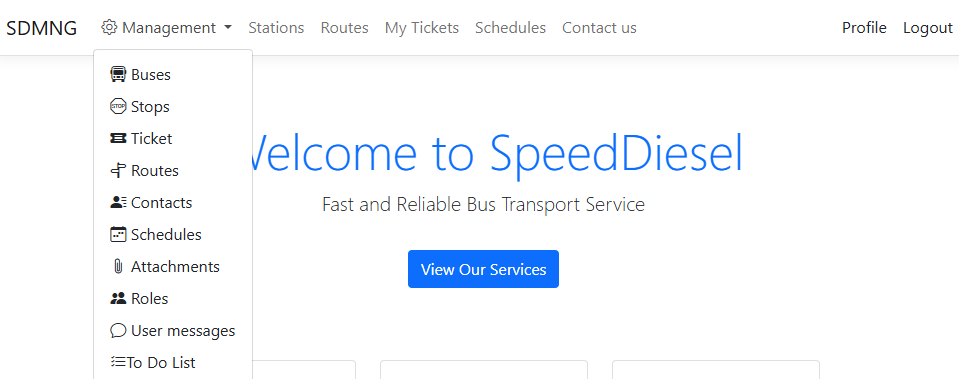
\includegraphics[width=1\textwidth]{Szakdolgozat/Mellekletek/navsavlogin1.PNG}
\caption{A navigációs sáv megjelenése bejelentkezett adminisztrátor számára.}
\label{fig:navsavlogged}
\end{figure}

A \ref{fig:navsavlogged}. ábrán a navigációs sáv bejelentkezett állapotban látható, adminisztrátori jogosultság mellett. Ebben az esetben a felhasználó számára elérhetővé válik egy további, legördülő menü, amely az adminisztrációs funkciókat csoportosítja. A menü tartalmazza többek között a megállók (Stops), buszok (Buses), útvonalak (Routes), menetrendek (Schedules), csatolmányok (Attachments), felhasználók (Contacts), jogosultságok (Roles), valamint teendők (ToDo List) kezelésére szolgáló linkeket. Ezek a nézetek csak az adminisztrátor szerepkörrel rendelkező felhasználók számára jelennek meg, és lehetőséget biztosítanak az alkalmazás teljes körű adatkezelésére és adminisztrálására. A menüsáv jobb oldalán továbbra is elérhető a kijelentkezési lehetőség, amely biztosítja a munkamenet megfelelő lezárását.

\subsubsection{Felhasználókezelési nézetek és résznézetek alkalmazása}

Az alkalmazásban a felhasználói azonosítással kapcsolatos funkciók – például a bejelentkezés, regisztráció, jelszócsere vagy email-ellenőrzés – dedikált nézeteken keresztül valósulnak meg, amelyek az \texttt{AccountController} vezérlőhöz kapcsolódnak. Ezek a nézetek a háttérben, ahogy már fentebb is említettem, a \texttt{Contact} nevű egyedi felhasználói modell adataira épülnek, amely az ASP.NET Identity \texttt{IdentityUser} osztályából származik.

A nézetek mindegyike külön ViewModel-t használ az űrlapadatok átadásához és validálásához. A \texttt{LoginViewModel}, \texttt{RegisterViewModel}, \texttt{VerifyEmailViewModel} és \texttt{ChangePasswordViewModel} mind külön-külön reprezentálják az adott funkcióhoz szükséges adatokat és a mezőkhöz kapcsolódó ellenőrzési szabályokat. A Razor-alapú nézetekben az \texttt{asp-for} és \texttt{asp-action} attribútumok biztosítják az adatkötést, valamint az automatikus hivatkozást a vezérlő megfelelő metódusaihoz.

Minden oldal egységes elrendezést követ, amelyet a \texttt{\_AccountLayout.cshtml} nézet biztosít. Ez a sablon definiálja az általános megjelenést, amelyet az összes hitelesítéssel kapcsolatos nézet örököl. Az űrlapok végén található \texttt{@section Scripts} blokk aszinkron módon betölti a \_ValidationScriptsPartial.cshtml nevű résznézetet, amely a kliensoldali validáláshoz szükséges JavaScript-függvényeket tartalmazza. Ennek köszönhetően a felhasználó azonnali visszajelzést kap a hibásan kitöltött vagy hiányzó mezőkről, még az adatküldés előtt.

Külön figyelmet érdemel a \texttt{\_LoginPartial.cshtml} résznézet szerepe, amely nem a hitelesítési nézeteken belül, hanem a főoldal elrendezésében, a navigációs sáv jobb oldalán jelenik meg. Ez a rész automatikusan lekérdezi a felhasználó hitelesítési állapotát, és dinamikusan változtatja a megjelenített tartalmat, amennyiben a látogató nincs bejelentkezve, megjelennek a „Login” és „Register” hivatkozások; ha viszont a felhasználó azonosítva van, akkor a felhasználónevet, valamint a kijelentkezési lehetőséget jeleníti meg.


\vspace{\baselineskip}
\subsubsection{Lista oldalak}
A listanézetek felépítése egységes, ahol az adott entitáshoz tartozó legfontosabb adatokat oszlopokban mutatjuk be. Minden ilyen nézet tartalmaz egy „Actions” nevű oszlopot is, amelyben három alapvető művelet található: a részletek megtekintése (Detail), az adat módosítása (Modify/Edit), valamint az elem törlése (Delete). Ezek a gombok minden egyes listaelem mellett megjelennek, és mindegyikhez az adott elem egyedi azonosítója (ID) van hozzárendelve. Ennek köszönhetően, amikor egy felhasználó rákattint valamelyik művelet gombra, a sornak vagy elemnek megfelelő oldalt nyitja meg, így biztosítva a pontos és gyors navigációt az funkciókat megvalósító oldalak között.

Az adminisztrátori feladatok kezelésére szolgáló nézet egy egyszerű táblázatos elrendezést használ, amely a \texttt{List<AdminTask>} típusú modell alapján jeleníti meg a rendszerben rögzített teendőket. A nézet elején a \texttt{@model} direktíva határozza meg, hogy milyen típusú adatot vár a nézet – jelen esetben az \texttt{AdminTask} típusú objektumokat tartalmazó listát.

A fejlécként szolgáló \texttt{ViewData["Title"]} meghatározza a lap címét, amely az oldal HTML fejlécében is megjelenik. Ezt követi egy főcím, valamint egy gomb a feladatok létrehozására (\texttt{Create}), amely egy \texttt{asp-action} segítségével a létrehozó űrlapra irányítja a felhasználót.

A feladatokat egy Bootstrap-alapú táblázat (\texttt{<table class="table">}) jeleníti meg. A \texttt{<thead>} rész a táblázat oszlopcímeit tartalmazza, amelyek sorrendben a feladat teljesítettségét jelző ikon, a cím, a határidő és a hozzárendelt műveletek.

A \texttt{<tbody>} részben egy \texttt{@foreach} ciklus segítségével iterálunk végig a modell objektumain. Minden egyes \texttt{AdminTask} típusú elem egy táblázatsorban (\texttt{<tr>}) kerül megjelenítésre. Az adott sor háttérszíne dinamikusan módosul: amennyiben a feladat már el van végezve (\texttt{IsResolved = true}), a sor \texttt{table-success} osztályt kap, ami zöld hátteret biztosít.

Az első oszlopban egy ikon jelenik meg, amennyiben a feladat már teljesített. Ez a Bootstrap Icons könyvtárból származik, és vizuálisan is jelzi az állapotot (\texttt{bi-check-circle-fill}). A második oszlop a feladat címét (\texttt{Title}), míg a harmadik a határidőt (\texttt{DueUntil}) jeleníti meg, rövid dátumformátumban.

Az utolsó oszlopban két gomb található: a „Details” gomb egy részletes nézetre navigál az adott feladattal kapcsolatban, míg az „Edit” gomb a módosító űrlaphoz visz. Mindkét hivatkozás dinamikusan kapja meg a feladat azonosítóját (\texttt{Id}) az \texttt{asp-route-id} attribútumon keresztül.

Ez a megközelítés nemcsak az adminisztratív feladatok kezelésére használható, hanem bármely entitástípus (például jegyek, útvonalak, felhasználók, csatolmányok) listázására is alkalmas. 


\subsubsection{Térképes megjelenítés a Stop részletező nézetben}
A megállók részletező nézete a felhasználói felület egyik fontos eleme, amely nemcsak szöveges információt nyújt a kiválasztott megállóról, hanem vizuálisan is segíti a tájékozódást egy interaktív térkép segítségével. A felület célja, hogy a felhasználó könnyen és gyorsan át tudja tekinteni egy adott megálló legfontosabb adatait, illetve annak pontos földrajzi elhelyezkedését.

A nézet az adott megálló objektum adatait jeleníti meg, amely a rendszerben egy Stop típusú modellként van definiálva. A megjelenített mezők közé tartozik a megálló neve, valamint annak szélességi és hosszúsági koordinátái. Ezek az értékek olvasható, de nem szerkeszthető formában jelennek meg, hogy a felhasználó ne tudjon véletlenül módosítani rajtuk.

A nézet különlegessége a térképes megjelenítés, amely a Leaflet nevű JavaScript-alapú térképkönyvtárra épül. Ez a könyvtár lehetővé teszi, hogy egy egyszerű, mégis interaktív térképet helyezzünk el az oldalon. A térkép automatikusan a kiválasztott megálló koordinátáira fókuszál, és egy jelölőt (marker) is elhelyez rajta, amely rámutat a pontos helyszínre. A jelölő fölé egy információs ablak is megnyílik, amelyben a megálló neve szerepel.

A megálló adatlap nézetében egy JavaScript-alapú megoldás jeleníti meg a megálló földrajzi elhelyezkedését térképen. Ennek célja, hogy a felhasználó pontosan lássa, hol található az adott megálló. A megvalósítás alapja az, hogy az adatmodellből (`Stop`) származó földrajzi koordináták (szélesség és hosszúság) JavaScript változókba kerülnek:

\begin{figure}[H]
\caption{Megálló helyének megjelenítése Leaflet térképen}
\label{fig:leaflet-stop-map}
\begin{minipage}{\textwidth}
\begin{BVerbatim}
var lat = @Html.Raw(Model.Latitude.ToString().Replace(',', '.'));
var lng = @Html.Raw(Model.Longitude.ToString().Replace(',', '.'));

if (!isNaN(lat) && !isNaN(lng)) {
    var map = L.map('stopMap').setView([lat, lng], 15);

    L.tileLayer('https://{s}.tile.openstreetmap.org/{z}/{x}/{y}.png', {
        maxZoom: 18
    }).addTo(map);

    L.marker([lat, lng])
        .addTo(map)
        .bindPopup("<strong>@Model.StopName</strong>")
        .openPopup();
}
\end{BVerbatim}
\end{minipage}
\end{figure}

\ref{fig:leaflet-stop-map}. ábrában szereplő JavaScript kódrészlet részletesen vázolja azt, hogyan épül fel a térképes megjelenítés. Az első két sor célja a Model.Latitude és Model.Longitude C\#-ban tárolt értékek JavaScript kompatibilis formátumra hozása. Mivel a magyar lokalizációban a tizedesjegy-leválasztó a vessző (','), ezeket előbb pontokra ('.') cseréljük le, hogy a Leaflet könyvtár által elvárt formátumot kapjuk meg.

Ezt követően egy ellenőrzés történik az isNaN() függvénnyel, amely megbizonyosodik arról, hogy a lat és lng változók valóban számértékek. Ha ez a feltétel teljesül, akkor a L.map() függvény inicializál egy új térképet a HTML oldalon elhelyezett stopMap azonosítójú <div> elemben. A setView() metódus beállítja a térkép középpontját a megadott koordinátákra, valamint egy nagyítási szintet, amely egy városi szintű részletességnek felel meg.

Ezután a L.tileLayer() függvény segítségével betöltjük az OpenStreetMap  térképelemet. Ez biztosítja az alapvető vizuális térképet, amelyre a marker rákerül. A betöltött réteg legnagyobb nagyítása maxZoom: 18, amely szintén a részletesség maximalizálását szolgálja.

Végül a L.marker() hívással létrehozunk egy új jelölőt a megálló pozíciójában. Az .addTo(map) metódus hozzáadja ezt a markert a térképhez. A .bindPopup() függvénnyel egy szöveges mezőt kapcsolunk hozzá, amely az aktuális megálló nevét jeleníti meg. Az .openPopup() metódus gondoskodik arról, hogy az információs buborék automatikusan megjelenjen a térképen, nem szükséges a felhasználónak rákattintania.

Ez az interaktív komponens tehát nem csupán egy vizuális kiegészítő, hanem jelentős mértékben hozzájárul a rendszer használhatóságához és felhasználóbarát jellegéhez. A JavaScript és a Leaflet könyvtár ilyen típusú alkalmazása egy modern, reszponzív felhasználói élményt eredményez, amely különösen hasznos lehet mobil vagy érintőképernyős eszközökön történő használat során is.

\subsubsection{Útvonal részletező nézet – több megálló vizuális megjelenítése térképen}

Az útvonal nézet működésében több ponton is párhuzamba állítható a megálló részletező felülettel: itt is térképes megjelenítés segíti a felhasználót, viszont a fókusz már nem egyetlen helyszín bemutatásán van, hanem egy egész megállósorozat áttekintésén. A nézet célja, hogy az útvonalhoz tartozó állomásokat sorrendben és valós helyükön mutassa be, azokat a térképen vizuálisan összekötve. Ezáltal a felhasználó nemcsak név szerint keresheti ki az egyes megállókat, hanem egy teljes képet kap arról, hogyan épül fel az adott útvonal.

Az útvonal nézet célja, hogy a felhasználó számára vizuálisan is értelmezhető módon mutassa be, hogyan épül fel egy adott járat – azaz milyen megállókat érint, és milyen sorrendben. A megvalósítás során a Leaflet könyvtárhoz kapcsolódó Routing Machine bővítményt használjuk, amely lehetővé teszi több pont összekötését és útvonal kirajzolását a térképen.

Minden megállóhoz először létrehozunk egy jelölőt (marker), amely az adott állomás koordinátáit használja, és egy rövid információs szöveget – jellemzően a megálló nevét – rendel hozzá. Ezek a jelölők segítik a felhasználót abban, hogy pontosan beazonosítsa az állomásokat:

\begin{figure}[H]
\caption{Jelölők és útvonalpontok elhelyezése a térképen}
\label{fig:route-markers}
\begin{minipage}{\textwidth}
\begin{BVerbatim}
var marker = L.marker([lat, lng]).addTo(map).bindPopup(stopName);
waypoints.push(L.latLng(lat, lng));
\end{BVerbatim}
\end{minipage}
\end{figure}

A \ref{fig:route-markers}. ábra kódrészlete azt mutatja, hogyan kerül fel egy új megálló a térképre, valamint hogyan tároljuk el az útvonal kirajzolásához szükséges koordinátákat egy waypoints nevű tömbbe. Ez a tömb minden egyes megállót reprezentál egy L.latLng() objektummal.

Miután az összes megálló bekerült ebbe a struktúrába, az útvonal grafikus megjelenítését a Leaflet Routing Machine végzi. A következő ábra szemlélteti a konfigurációs lehetőségeket:

\begin{figure}[H]
\caption{Útvonal kirajzolása Leaflet Routing Machine segítségével}
\label{fig:routing-control}
\begin{minipage}{\textwidth}
\begin{BVerbatim}
L.Routing.control({
waypoints: waypoints,
lineOptions: {
styles: [
{ color: '#FF1493', weight: 6, opacity: 0.95 },
{ color: '#FFFFFF', weight: 2, opacity: 1 }
]
},
createMarker: function() { return null; },
routeWhileDragging: false
}).addTo(map);
\end{BVerbatim}
\end{minipage}
\end{figure}

A \ref{fig:routing-control}. ábrában látható konfigurációs blokk részletezi az útvonal megjelenítésének beállításait. A lineOptions szekcióban több színt és vastagságot rendelhetünk a kirajzolt útvonalhoz, ezzel vizuálisan is kiemelve azt. A createMarker opció null értékre van állítva, mivel a marker-ek már korábban, kézzel kerültek felhelyezésre, és itt nem kívánunk duplikációt.

Az utolsó lépés a térkép automatikus igazítása az útvonal teljes hosszára. Ezt a fitBounds() függvénnyel érjük el.

\begin{figure}[H]
\caption{Térkép igazítása az összes megálló alapján}
\label{fig:fit-bounds}
\begin{minipage}{\textwidth}
\begin{BVerbatim}
map.fitBounds(L.latLngBounds(waypoints));
\end{BVerbatim}
\end{minipage}
\end{figure}

A \ref{fig:fit-bounds}. kódrészlet garantálja, hogy a térkép minden megállót megjelenítsen, anélkül, hogy a felhasználónak manuálisan kellene mozgatnia vagy nagyítania a nézetet. Ez különösen akkor hasznos, ha az útvonal hosszú és több városrészt érint.

Összességében ez a funkció nem csupán egy hasznos kiegészítő, hanem egy olyan kulcsfontosságú elem, amely a vizualizáció erejével támogatja a közlekedési információk gyors és intuitív értelmezését. A felhasználó egy pillantással áttekintheti az útvonal struktúráját, így biztosabban dönthet az utazási lehetőségekről.


\subsubsection{Ticket detail page }

A  \ref{fig:ticket-detail-kolozsvar-torda}. ábrán látható jegyrészletező oldal, a projekt szempontjából kiemelt jelentőséggel bír, hiszen ez az a funkció, amely az egész alkalmazás ötletét elindította. A kezdeti elképzelés abból született, hogy a felhasználók számára egy olyan felületet biztosítsunk, ahol a megvásárolt jegyük minden lényeges információja egyetlen, jól átlátható nézetben elérhető.

Az oldal szere, hogy minden olyan információt tartalmazzon, ami az utazás szempontjából fontos lehet. Megjelenik rajta a járat neve, az ahhoz tartozó busz rendszáma, a lefoglalt ülőhely száma, valamint az indulási és érkezési időpontok, illetve azok helyszínei. Ezen adatok strukturált formában kerülnek megjelenítésre, így a felhasználó egy pillantással át tudja tekinteni a foglalás részleteit.

Ami azonban igazán megkülönbözteti ezt a felületet más rendszerektől, az a térképes integráció. A nézet közvetlenül tartalmazza az utazás útvonalát is, amely egy térképen jelenik meg, vizuálisan kirajzolva a megállók közötti kapcsolatokat. Ennek óriási előnye, hogy a felhasználónak nem kell külön oldalakon keresgélnie, vagy új ablakot megnyitnia annak érdekében, hogy földrajzi képet kapjon az útvonalról – az interaktív térkép közvetlenül a jegyadatok mellett helyezkedik el, így a kétféle információ egy helyen, egymást kiegészítve jelenik meg. A megvalósítása teljes mértékben megegyezik az útvonal nézet alfejezetben leírt lépésekkel, amint a megállókat a feldolgoztam, majd későbbiekben kirajzoltam az interaktív térképes felületen.

Ez a megközelítés nemcsak kényelmi szempontból előnyös, hanem a felhasználói élmény szempontjából is kulcsfontosságú. A rendszer úgy lett kialakítva, hogy a legfontosabb információkat – akár időbeli, akár térbeli adatokról legyen szó – egyetlen oldalon tegye elérhetővé, ezzel is minimalizálva a felesleges navigációt és az információk keresésére fordított időt. Mindez nem csupán praktikus, hanem szemléletformáló is: a projekt középpontjába magát az utazó embert helyezi, és a lehető legkényelmesebb módon szolgáltatja számára a szükséges adatokat.

\begin{figure}[H]
    \centering
    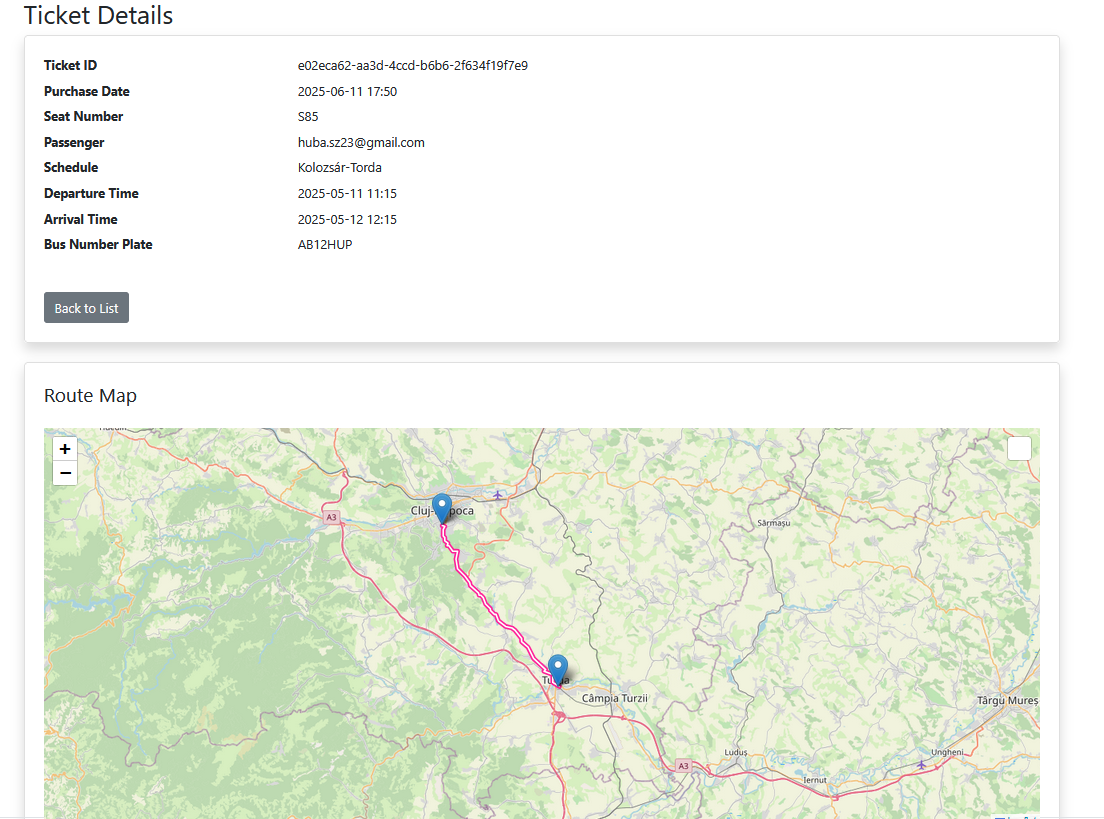
\includegraphics[width=0.9\textwidth]{Szakdolgozat/Mellekletek/ticketdetail.PNG}
    \caption{Kolozsvár–Torda útvonalra vásárolt jegy részletező nézete. Az oldalon jól látható a járat neve, a busz rendszáma, az ülőhely száma, az indulási és érkezési időpontok és helyszínek, valamint a teljes útvonal térképes megjelenítése.}
    \label{fig:ticket-detail-kolozsvar-torda}
\end{figure}


